% -*- TeX-master: "main"; fill-column: 72 -*-

\newpage
\section{HARMONY: proposed extensions 2018}

\begin{quote}
 \textbf{\Large The contents of this section are, as yet, unofficial and are formulated here in order to optimize spec development effort.}
\end{quote}

The proposed \FBCPackage version~3 extends the definition of the \FluxObjective, extends the definition of the \token{chemicalFormula}, defines a \UserConstraint and adds a generic \KeyValuePair annotation.

\begin{figure}[ht!]
  \centering
  % Requires \usepackage{graphicx}
  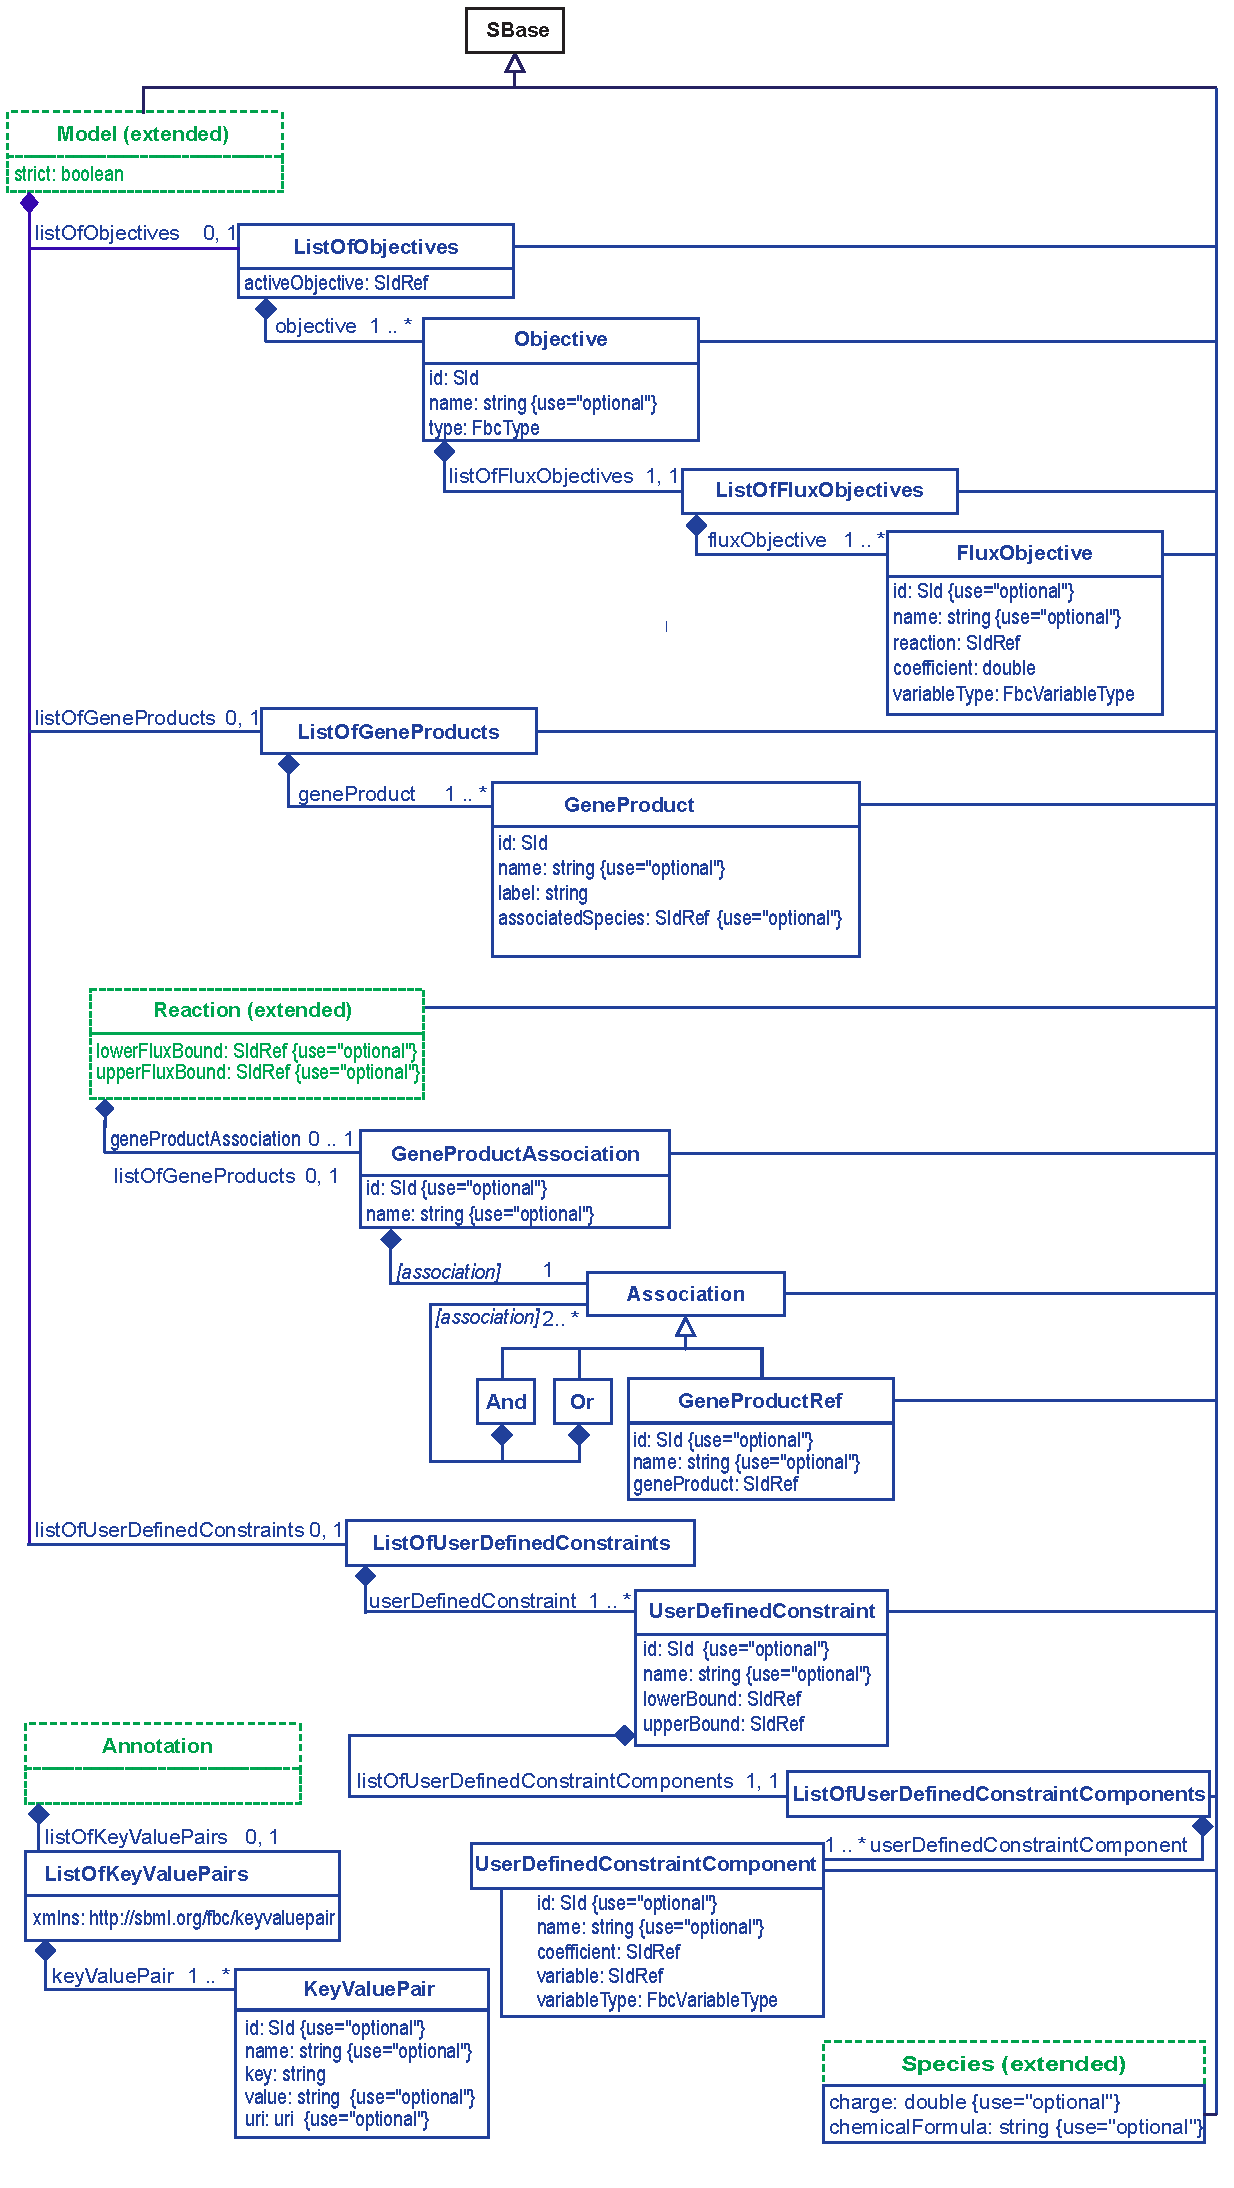
\includegraphics[height=0.85\textheight]{images/fbc_uml_v3.pdf}\\
  \caption{A UML representation of the \FBCPackage version three. Derived from \SBase, most\FBC classes inherit support for constructs such as SBML \Notes and \Annotation's. The [association] element name is the name of the class, de-capitalized. In this case, the possible values are "and", "or", or "geneProductRef". See \ref{conventions} for conventions related to this figure. The individual classes are further discussed in the text.}
  \label{fig:fbc_uml_v3}
\end{figure}

%\subsection{The extended \class{SBase} class}
%\label{sbase-class-kv}

\subsection{The extended \class{Model} class}
\label{model-class-kv}
%\label{listoffluxbounds-class}

The \SBML \Model class is extended by a \token{listOfUserConstraints} of which it may contain at most one.
%
\begin{figure}[ht]
  \centering
  % Requires \usepackage{graphicx}
  %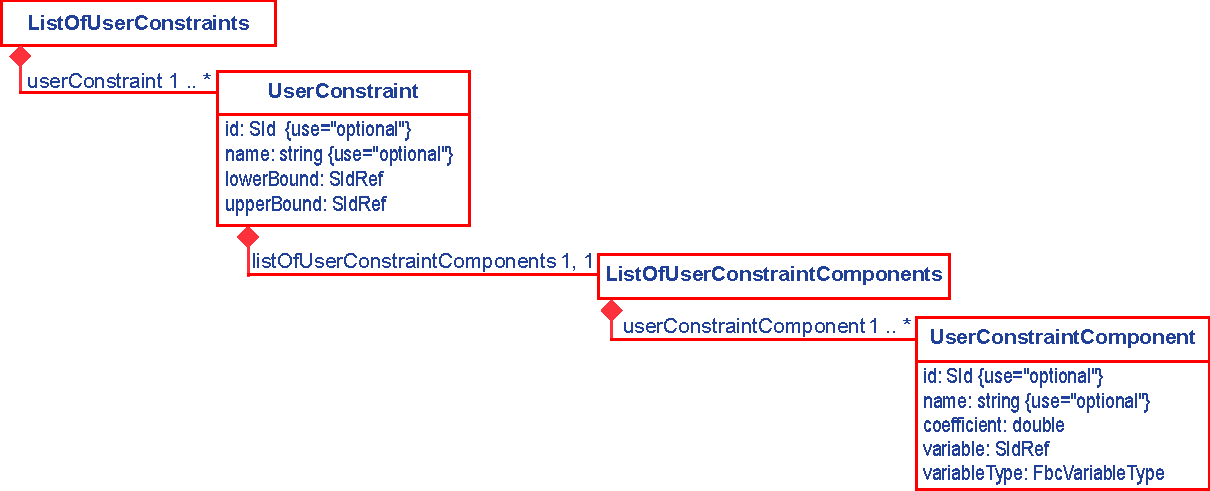
\includegraphics[width=6cm]{images/fbc_v3_uml_userconstraint.pdf}\\
  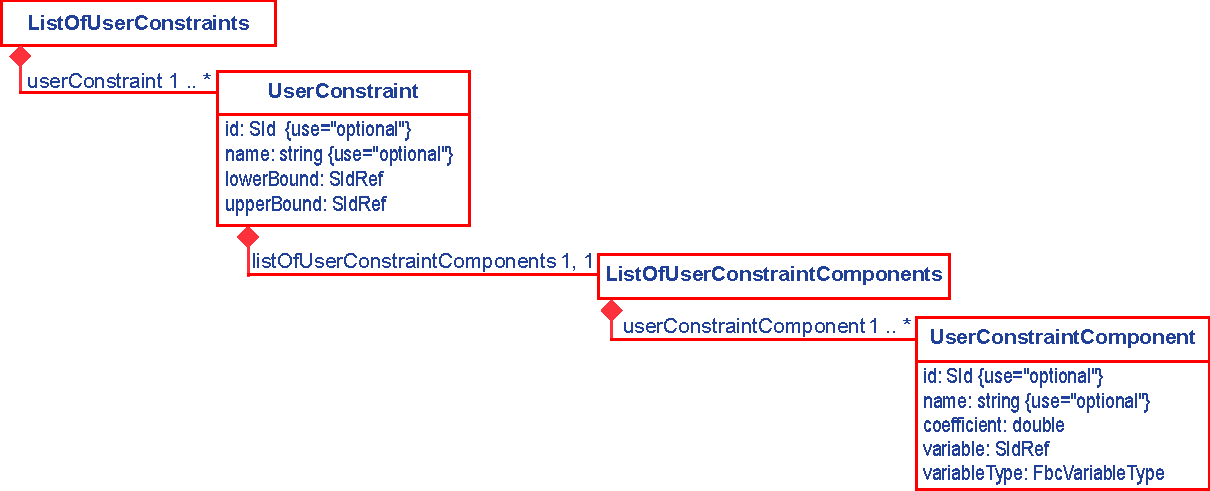
\includegraphics[width=\textwidth]{images/fbc_v3_uml_userconstraint.pdf}\\
  \caption{A UML representation of the \SBML \Model class extended in
  the \FBCPackage by the \ListOfUserConstraints. See \ref{conventions} for conventions related to this figure.}
  \label{fig:fbc_v3_uml_user_constraints}
\end{figure}

\subsubsection{Type \primtypeNC{FbcVariableType}}
\label{primtype-fbcvariabletype}

The \FBCPackage defines a new enumerated type \primtype{FbcVariableType} which
represents the index of a variable that occurs in either the \FluxObjective or \UserConstraintComponent. It has one of the following two values, \val{linear} or \val{quadratic}.


%\subsubsection{Type \primtypeNC{FbcUCCVariableType}}
%\label{primtype-fbcuserconstraintvariabletype}
%
%The \FBCPackage defines a new enumerated type \primtype{FbcUCCVariableType} which
%represents the index of a variable that occurs in a user defined constraint. It can have one
%of the following two values \val{linear} or \val{quadratic}.

\subsubsection{The \FBC \class{listOfUserConstraints}}
\label{listofuserconstraints-class}

As shown in \ref{fig:fbc_v3_uml_user_constraints} the \ListOfUserConstraints is derived from \SBase and inherits the attributes \token{metaid} and \token{sboTerm}, as well as
the subcomponents for \Annotation and \Notes. The \ListOfUserConstraints must contain at least one \UserConstraint (defined in \ref{userconstraint-class}).

\subsection{The extended \class{Species} class}

\paragraph{The \token{chemicalFormula} attribute}
\label{chemicalFormula-attribute}

The optional attribute \token{chemicalFormula} containing a \primtype{string} that represents the \Species objects elemental composition.
%
\exampleFile{examples/ex-v3-species.txt}
%
\newtxt{While there are many ways of referring to an elemental composition, the purpose of the \token{chemicalFormula} attribute is to enable reaction balancing and validation, something of particular importance in constraint-based models.}

\newtxt{The format of the \token{chemicalFormula} should, whenever possible, consist only of atomic names
(as in the Periodic Table). Similarly, for enhanced inter-operability, the element order should be arranged according to the Hill system} \citep{hillsystem, hillwikipedia}.
%
\begin{table}[h!]
  \begin{tabular}{ccc}
    % after \\: \hline or \cline{col1-col2} \cline{col3-col4} ...
     $H_{2}O_{4}S$ & $C_{2}H_{5}Br$ & $BrH$ \\
     $C_{10}H_{12}N_{5}O_{13}P_{3}$ & $CH_{3}I$ & $CH_{4}$  \\
  \end{tabular}
  \caption{Examples of chemical formulas written using the Hill System. As
	described in \ref{chemicalFormula-attribute}}\label{table:hill}
\end{table}
%
\newtxt{Using this notation the number of carbon atoms in a molecule is indicated first, followed by the number of hydrogen atoms and then the number of all other chemical elements in alphabetical order. When the formula contains no carbon; all elements, including hydrogen, are listed alphabetically. Where there is more than a single atom present, this is indicated with an integer that precedes the element symbol.}

\newtxt{However, in certain situations it does become necessary to use a generic symbol in a user defined compound. For example, such symbols can include \textsf{R} and \textsf{X} and have the general form of a single capital letter followed by zero or more lowercase letters."}
%
\begin{table}[h!]
  \begin{tabular}{ccc}
    % after \\: \hline or \cline{col1-col2} \cline{col3-col4} ...
     $RCONH_{2}$ & $RCOX$ & $C_{2}H_{4}O_{2}(CH_{2})_{n}$ \\
  \end{tabular}
  \caption{Examples of chemical formulas written using allowed non-Hill symbols, as described in \ref{chemicalFormula-attribute}.}\label{table:non-hill}
\end{table}
%
\newtxt{In addition, the undefined parenthesised group index may also be used, $(\ldots)_n$. Note the $n$ here has a literal intepretation and cannot be replaced by a value $(\ldots)_2$ or form part of an expression, $(\ldots)_{n-1}$.}

\newtxt{While not invalid, the use of \textsf{R}, \textsf{X} and $(\ldots)_n$ is not encouraged as, in general, any \Reaction in which such a \Species occurs as a reagent cannot be balanced. Therefore, any \token{chemicalFormula} that contains any of the aforementioned, non-Hill compatible symbols will generate a `best practices' warning on model validation.}

\subsection{The \FBC \class{FluxObjective} class}

The \FBC \FluxObjective class is derived from \SBML \SBase and inherits
\token{metaid} and \token{sboTerm}, as well as the subcomponents for
\Annotation and \Notes.
%
\begin{figure}[ht]
  \centering
  % Requires \usepackage{graphicx}
  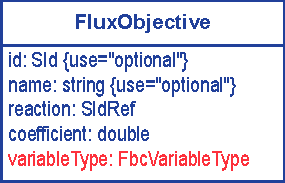
\includegraphics[width=6cm]{images/fbc_v3_uml_fobj.pdf}\\
  \caption{A UML representation of the \FBCPackage \FluxObjective class. For a complete description see \ref{fig:fbc_uml} as well as \ref{conventions} for conventions related to this figure.}
  \label{fig:fbc_uml_userconstraint}
\end{figure}
%
The \FluxObjective class is a relatively simple container for a model
variable that can be expressed as a `linear' or `quadratic', weighted by a signed linear coefficient.

\paragraph{The \token{id} and \token{name} attributes}
A \FluxObjective has two optional attributes: \token{id} an attribute of
type \primtype{SId} and \token{name} an attribute of type \primtype{string}.

\paragraph{The \token{reaction} and \token{coefficient} attributes}
The required \token{reaction} is of type \primtype{SIdRef} and is restricted
to refer only to a \Reaction while the \token{coefficient} attribute
holds a \primtype{double} referring to the coefficient that this \FluxObjective
takes in the enclosing \Objective. 

\newtxt{\paragraph{The \token{variableType} attribute}
The required \token{variableType} attribute contains a \primtype{FbcVariableType} that
represents the index of a variable that occurs in a \FluxObjective. It can have one
of the following two values \val{linear} or \val{quadratic}.}

\paragraph{Flux objectives: example code}
\newtxt{An objective with purely linear terms in LP format:} \verb"Maximize: 1 R1 + 2 R2"
%
\exampleFile{examples/ex-v3-fluxobjective-linear.txt}
%
\newtxt{Similarly, an objective with a quadratic term in LP format:} \verb"Minimize: 1 R1 + [4 R2^2]/2"
%
\exampleFile{examples/ex-v3-fluxobjective.txt}

\paragraph{Units}
As described above the \FluxObjective defined here as $n\cdot J$ where
the \token{coefficient} ($n$) is dimensionless and the \token{value} ($J$)
takes the units of the \token{reaction} flux i.e.,~``extent per time''.
Therefore, the \FluxObjective ($n\cdot J$)  has the unit ``extent per time''
where the units of reaction ``extent'' and ``time'' are defined globally. 







\subsection{The \FBC \class{UserConstraint} class}
\label{userconstraint-class}

The \FBC \UserConstraint class is derived from \SBML \SBase and inherits
\token{metaid} and \token{sboTerm}, as well as the subcomponents for
\Annotation and \Notes. It's purpose is to define non-stoichiometric constraints, i.e., constraints that are not implicitly defined by the reaction network. The \UserConstraint contains a linear combination of \UserConstraintComponent's contained in a \ListOfUserConstraintComponents.

\paragraph{The \token{id} and \token{name} attributes}
A \UserConstraint has an optional \token{id} of type
\primtype{SId} and an optional attribute \token{name} of type \primtype{string}.

\paragraph{The \token{lowerBound} attribute}
The required \token{lowerBound} attribute contains an \primtype{SIdRef} that references a \Parameter which contains the lower boundary value of the \UserConstraint.

\paragraph{The \token{upperBound} attribute}
The required \token{upperBound} attribute contains an \primtype{SIdRef} that references a \Parameter which contains the upper boundary value of the \UserConstraint.

\paragraph{The \token{listOfUserConstraintComponents} element}
\label{listofuserconstraintcomponents-class}

The element \token{listOfUserConstraintComponents} which contains a
\ListOfUserConstraintComponents is derived from and functions like a typical \SBML
\textsf{\textbf{ListOf\rule{0.15in}{0.5pt}}} class with the restriction that it
must contain one or more elements of type \UserConstraintComponent (see \ref{userconstraintcomponent-class}).
This implies that if a \UserConstraint is defined there should be at least
one \UserConstraintComponent contained in a \ListOfUserConstraintComponents.
%
\exampleFile{examples/ex-v3-userconstraints.txt}


%\begin{figure}[ht]
%  \centering
%  % Requires \usepackage{graphicx}
%  %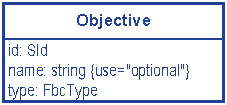
\includegraphics[width=5cm]{images/v2harmony_fbc_objective.pdf}\\
%  \caption{A UML representation of the \FBCPackage \UserConstraint class. For a complete description see \ref{fig:fbc_uml} as well as \ref{conventions} for conventions related to this figure.}
%  \label{fig:fbc_uml_userconstraint}
%\end{figure}

\subsection{The \FBC \class{UserConstraintComponent} class}
\label{userconstraintcomponent-class}

The \FBC \UserConstraintComponent class is derived from \SBML \SBase and inherits
\token{metaid} and \token{sboTerm}, as well as the subcomponents for
\Annotation and \Notes. The \UserConstraintComponent class is a relatively simple container for a variable and a variable type specifier which is weighted by a signed coefficient.

\paragraph{The \token{id} and \token{name} attributes}
An \UserConstraintComponent has an optional \token{id} of type \primtype{SId} and an optional attribute \token{name} of type \primtype{string}.

\paragraph{The \token{coefficient} attribute}
The required \token{coefficient} attribute contains an \primtype{SIdRef} that is restricted to reference only a \Parameter which then holds the coefficient value. (\newtxt{In strict mode this should behave like a \FluxObjective coefficient for example, be defined as constant and not able to have the value NaN or $\pm$inf }).

\paragraph{The \token{variable} attribute}
The required \token{variable} attribute contains an \primtype{SIdRef} that is restricted to reference the \primtype{SId} of either a \Reaction or (\newtxt{non-constant}) \Parameter. \newtxt{If a \token{variable} refers to a non-constant \Parameter, it may not refer to an \primtype{SId} referenced by a \token{coefficient} attribute.} {\textbf{\large BGO: or more generally should parameters that act as variables only then be available to be referenced as variables (not coefficients, bounds etc)?}}

\paragraph{The \token{variableType} attribute}
The required \token{variableType} attribute contains a \primtype{FbcVariableType} that indicates whether a variable should be considered as `linear' or `quadratic'.


\subsection{The \FBC \class{ListOfKeyValuePairs} class}
\label{listofkeyvaluepairs-class}

The \ListOfKeyValuePairs, see \ref{fig:fbc_v3_uml_keyvalue} for details, forms the basis of a controlled annotation defined by the \FBCPackage. This element defines a `structured note' or `descriptive list' of keys and associated values.
%
\exampleFile{examples/ex-v3-kvp1.txt}
%
%\begin{quote}
%\begin{description}
%  \item[keyX] 47
%  \item[ZZkey] beard level 5
%  \item[x--factor] intangible metaphysical property
%\end{description}
%\end{quote}
%%
As such it is analogous to the official \SBML RDF annotation used to support MIRIAM annotations, as defined in the \SBML specification documents. Similarly, we define an official \FBC annotation, the \ListOfKeyValuePairs. The advantages of using the existing \SBML annotation mechanism include, \SBase not needing any further extension (a technical/performance advantage) and the annotation can be used directly in all existing \SBML levels and versions.

As is the case with the RDF/MIRIAM annotations, support for \ListOfKeyValuePairs will be included in the \SBML support libraries.
%
\begin{figure}[ht]
  \centering
  % Requires \usepackage{graphicx}
  %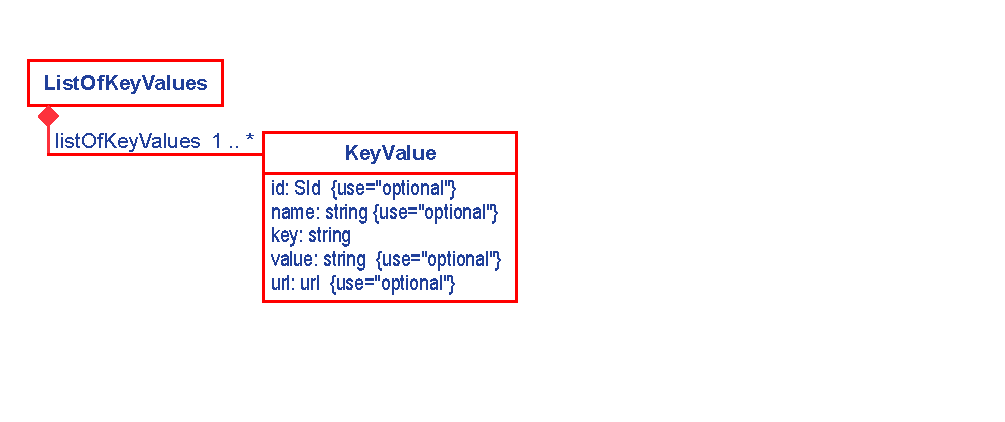
\includegraphics[width=6cm]{images/fbc_v3_uml_keyvalue.pdf}\\
  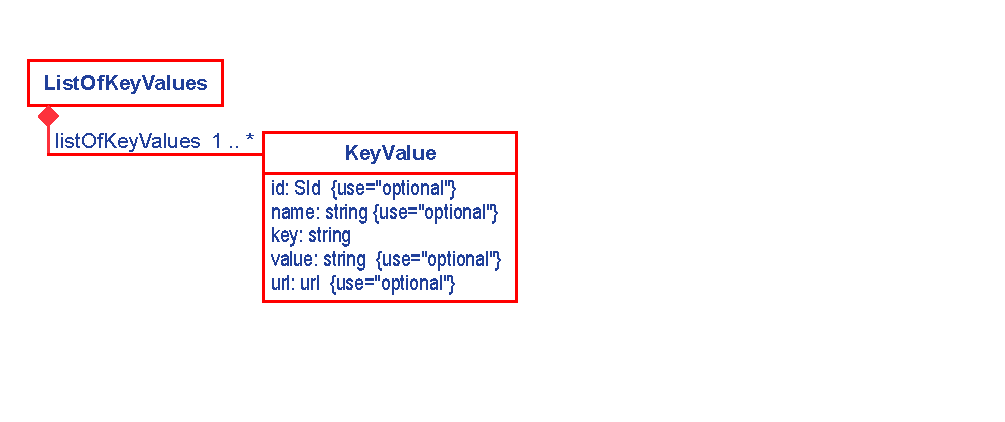
\includegraphics[width=0.6\textwidth]{images/fbc_v3_uml_keyvalue.pdf}\\
  \caption{A UML representation of the \SBML \SBase class extended in
  the \FBCPackage by the \protect{\ListOfKeyValuePairs}. See \ref{conventions} for conventions related to this figure.}
  \label{fig:fbc_v3_uml_keyvalue}
\end{figure}
%
As shown in \ref{fig:fbc_v3_uml_keyvalue}, the \ListOfKeyValuePairs is derived from and functions like a typical \SBML \textsf{\textbf{ListOf\rule{0.15in}{0.5pt}}} class with the restriction that it must contain one or more elements of type \KeyValuePair (see \ref{keyvaluepair-class}). In addition it defines a single mandatory attribute, \token{xmlns}, which identifies the annotation as belonging to the \FBCPackage.

\paragraph{The \token{xmlns} attribute}
The \token{xmlns} is a mandatory component of the \ListOfKeyValuePairs, is of the type \primtype{url} which must have the value \token{http://sbml.org/fbc/keyvaluepair}. 


\subsection{The \FBC \class{KeyValuePair} class}
\label{keyvaluepair-class}

The \FBC \KeyValuePair class is not derived from \SBase and therefore \newtxt{does not} inherit \token{metaid} and \token{sboTerm}, as well as, the subcomponents for
\Annotation and \Notes. It's purpose is to define a key--value pair with an extended key definition.

The \KeyValuePair defines a single mandatory attribute the \token{key} as well as two optional attributes: \token{value} and \token{url}.

\paragraph{The \token{key} attribute}
The \token{key} is the mandatory component of the \KeyValuePair pair and is of type \primtype{string}. It has the special property that every \token{key} in an enclosing \ListOfKeyValuePairs must be unique.

\paragraph{The \token{value} attribute}
The optional \token{value} attribute is of \primtype{string} and contains the value associated with a particular \token{key}. If not present, the \KeyValuePair is defined to have no value.

\paragraph{The \token{url} attribute}
The optional attribute \token{url} is of type \primtype{url}. This attribute is included and references a resource that contains a description of the \token{key} component of the \KeyValuePair. Note that the nature or structure of this resource is not defined. For example, it could be an HTML page with a textual description of the \token{key}(s) used by a particular tool or another that contains a table of key definitions. A theoretical example of a resource, as used in the above example, can be found here: \url{http://www.bgoli.net/kvp/propdefs1}

However, the concomitant development of a central \token{key} resource and associated standardised \token{key} definition would enable greater model reusability and tool interoperability and be of benefit to the broader \SBML community.




